\chapter{Background and Related Work}
\label{cha:background}
In this chapter we introduce the background and motivation for this project, and related work in the area. A summary of each section is given below.

\begin{itemize}
    \item Section \ref{sec:motivation}: This section details the main motivation for the project, including potential areas of application.
    \item Section \ref{sec:comp}: Here we introduce Compositional Data, outlining examples and areas of application. We then present the current methods used in the analysis of this data. 
    \item Section \ref{sec:dimred}: This section presents the topic of dimensionality reduction. We introduce the most common algorithm, PCA, as well as methods specific to compositional data. We also present several examples to illustrate the advantages of the different approaches.  
    \item Section \ref{sec:sup}: The main applications of supervised learning, regression and classification, are introduced here. 
\end{itemize} \pagebreak

\section{Compositional Data}
\label{sec:comp}

\subsection{Definition}
As stated earlier, compositional data consists of a set of non-negative vectors which sum to a constant value (this is usually normalised to be 1 so the components can be interpreted as percentages of a whole). Formally, a compositional matrix $\mathbf{X} \in \mathbb{R}^{n\times d}$ will have each row vector $x_i \in \mathbb{R}^d$ as an element of the $d-1$ dimensional simplex, which is defined as: $$S^{d-1} = \{s \in \mathbb{R}^d : \sum_{i=1}^{d}s_i = c\}$$ for a fixed constant $c$ (that is, each column vector $x_i$ must sum to $c$). We note that the simplex is of dimension $d-1$ because we can determine the final component from the sum of the rest, given that $c$ is a fixed constant. More precisely, the final component of a compositional vector $x_i$ is clearly $(x_i)_{d} =  c - \sum_{j=1}^{d-1}(x_i)_j$ and so $x_i$ is of dimension $d-1$.   


\subsection{Example: RGB and the 2D simplex}
An example which illustrates this concept well is the RGB triangle. Any colour in RGB format can be interpreted as a composition of each of the colours Red, Green and Blue. In the notation above, this corresponds to a vector in $\mathbb{R}^3$.
Figure \ref{fig:rgbsimplex} gives a visual representation of the simplex of all such vectors. 

\usetikzlibrary{fadings}
\begin{figure}
 \begin{center}
\subfigure[An RGB Colour Triangle is an example of a 2D simplex in 3D space]{  
   
       \begin{tikzpicture}
      \fill[green] (90:4) -- (210:4) -- (-30:4) -- cycle;
      \fill[blue,path fading=west] (90:4) -- (210:4) -- (-30:4) -- cycle;
      \fill[red,path fading=south] (90:4) -- (210:4) -- (-30:4) -- cycle;
    \end{tikzpicture}
}

\subfigure[The standard 2D simplex as a subset of $\mathbb{R}^3$. The shaded region corresponds to the set $S^{2} = \{\mathbf{x} \in \mathbb{R}^3 : x_1 + x_2 + x_3 = 1\}$]{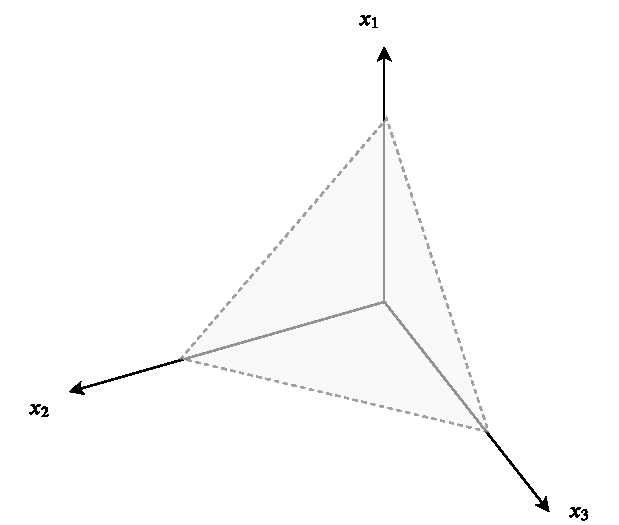
\includegraphics[]{figs/2dsimplex(2)(1).pdf}}

    \caption{The 2D Simplex}
    \label{fig:rgbsimplex}
    
\end{center}
\end{figure}




Using this example, we note several points: 
\begin{itemize}
    \item The total magnitude of the vector $(R,G,B)$ is irrelevant to the colour produced. What is important it the relative magnitudes between the values $R,G,B$. This is why we can normalise compositions to $1$ without losing or distorting information.   
    \item The simplex is fully defined as a 2D subset of $\mathbb{R}^3$, as it is a triangle. In general, the simplex extends the triangle to higher dimensions.  
    \item The maximum value any of $R,G,B$ can take is given by each of the vertices.
    \item A gain in any particular $R,G,B$ will correspond to that amount lost between the other values. This is the qualitative interpretation of the restriction that the parts must sum to a fixed value. 
\end{itemize}
\pagebreak



 
\subsection{Compositional Data Analysis (CoDA)}
\label{coda}
Given compositional data lies on the simplex, analysis of these data are complicated by the fact that they exist in a non-Euclidean mathematical space. As such, any attempt to compare distances between elements of this space cannot take place in the standard manner. The study of Compositional Data is known as Compositional Data Analysis (CoDA for short) and \cite{Aitchison1982} was the first to treat this issue in depth. At the core of Aitchinson's approach was the idea of a log transformation. For a point on the simplex, applying such a transformation embeds the point in Euclidean space, facilitating standard distance comparisons. There are several of these transformations, however they lead to similar results as they only differ by a linear transformation. The most widely used (and most applicable for this project) is the centered log ratio (clr) transformation. Using notation from \cite{Avalos2018}, the clr transformation is formally defined as: $$\mathbf{c}_{KL}(\mathbf{x}) = \log \left(\frac{x}{(\prod_{j=1}^d x_j)^{\frac{1}{d}}}\right)$$  

We note that $\mathbf{c}_{KL} : S^{d-1} \to  \mathbb{R}^d$ is a bijective map from $S^{d-1}$ to  $\mathbb{R}^d$ by observing the inverse function which is given by 
$$\mathbf{c}_{KL}^{-1}(\mathbf{x}) = e^\mathbf{x} \prod_{i=1}^d e^{\frac{x_j}{1-d}}$$

It follows that this embedding gives a unique value in $\mathbb{R}^d$ for all elements in the simplex $S^{d-1}$. The analysis of the embedded data can therefore be conducted using standard methods without any loss of information. \\

The standard methodology for modern practitioners is to use the analysis of this log transformed data, and relate the conclusions made in the transformed space back to the original domain \citep{Aitchison2003}. This approach is more mathematically grounded than simply using standard methods in the simplex, but still leads to several issues. There are problems with translating interpretations from the new coordinate system back to the original domain. We cannot draw conclusions about the absolute magnitude of quantities, as compositions are inherently relative. We will soon see that the log transformation may also fail to capture relationships in the original domain (Section \ref{codapca}). There have been some attempts to improve upon CoDA techniques, such as hypersphere transformations \citep{} and Dirichlet models \citep{}. As discussed by \cite{}, the hypersphere approach is not fully justified mathematically. Similarly, Dirichlet models make unrealistic assumptions on the data. These issues help justify the need for further research in the area. 

\section{Dimensionality Reduction}
\label{sec:dimred}

A concept crucial to this thesis is dimensionality reduction. Broadly, this refers to the set of techniques used to represent high dimensional data in a reduced form. Formally, we consider a data matrix $X \in \mathbb{R}^{d \times n}$ with $n$ elements, each with dimension $d$. The goal of dimensionality reduction is then to find what we denote as a representation matrix $A \in \mathbb{R}^{l \times n}$, where $l < d$. Since $l < d$, each column $x_i \in \mathbb{R}^d$ of $X$ will map to a lower dimensional representation $a_i \in \mathbb{R}^l$. This can be interpreted as projection of $x_i$ to a new coordinate system. In practice, it can be useful to consider $A$ as an encoding of $X$. We can then reconstruct an approximation to the original matrix $X$ through a decoding matrix $V \in \mathbb{R}^{l \times d}$. Through this we can obtain a reconstruction of $X$ of the same dimension, which is given by $V^TA \in \mathbb{R}^{d \times n}$. \\

Dimensionality reduction is useful for several reasons: \citep{Shlens2005}: 

\begin{itemize}
    \item The use of a low level representation of the data leads to smaller memory footprint and quicker algorithms 
    \item The dimensions which are removed often represent noise in the data, making it easier to find relationships between variables
    \item When dimensions are highly correlated, changing the coordinate space can remove redundancy
    \item Taking the low level dimension $l \leq 3$ allows for visualisation of higher dimensional data
\end{itemize}

There are many different approaches to dimensionality reduction, which seek to find $A$ based on different criteria and assumptions on the underlying data $X$. These approaches can be considered as minimising a distortion (generalised distance)  between functions of the reconstruction $V^TA$ and the orignal matrix $X$. This interpretation was particularly helpful for the paper which inspired this project \citep{Avalos2018}. Below we outline those dimensionality reduction techniques relevant to this research.    

\subsection{Principal Component Analysis (PCA)}
The most well known dimensionality reduction method is Principal Component Analysis (PCA) \citep{MackiewiczRatajczak1993}. There are several derivations and interpretations of PCA, with all giving the same final result. An intuitive explanation is given by \cite{Shlens2005}, which we draw from to explain the concept. PCA seeks to find a representation matrix $A$ where the covariance matrix of $A$ is diagonalised. As explained by \cite{Shlens2005}, this is desirable as each basis vector for the new coordinate system is uncorrelated, which minimises the shared information between them. Furthermore, PCA chooses the first basis $\mathbf{v}_1$ of the transformation $\mathbf{V}$ as the direction with maximum variance. The next basis is taken to be the direction with largest variance orthogonal to $\mathbf{v}_1$. This process continues, with $\mathbf{v}_i$ being the direction of maximum variance orthogonal to the subspace spanned by $\mathbf{v}_1, ...,\mathbf{v}_{i-1}$... derivation with $A = VX$... ($X = V^{-1}A = V^TA$, only when deleting dimensions becomes an approximation. $V$ acts only as a rotation to express $X$ in terms of an orthonormal basis) 


The process used to find the orthonormal basis in PCA is the Gram-Schmidt \ref{} algorithm. It is also used to compute the Singular Value Decomposition (SVD) of a matrix \ref{}. This is why the SVD can be used to find the PCA projection matrix. The SVD has been highly optimised in many current software packages, and so it is used in practice to compute the projection $V$ given by PCA.  

Add diagram/example! (2D gaussian, data projected onto 1D?)


\subsection{Exponential Family PCA}
Exponential family PCA: Extends PCA analogous to GLMs extending Linear Regression to exponential family. In the same way, allows for loss functions which are more appropriate for the parameter space, where parameters can be non Gaussian. Main example is count data i.e. Poisson which is exponential family. Situation is when data space (e.g. Poisson) is different to parameter space e.g. Reals

\subsection{CoDA-PCA}
\label{codapca}
This thesis primarily builds upon the 2018 NIPS paper on Representation Learning for Compositional Data \citep{Avalos2018}. The main result of the paper is the algorithm CoDA-PCA, which is a method for dimensionality reduction of compositional data. The standard approach to dimensionality reduction prior to this result was to apply PCA to the clr transformed data. CoDA-PCA combines clr with exponential family PCA, which allows PCA to be applied to count data. This simultaneously keeps the data centered through clr, and makes use of a loss function which considers the count nature of the data in the reconstruction error. The improvement can be seen dramatically in the ARMS example presented in the paper, where we see that CoDA-PCA and its variants are the only algorithms which faithfully represent the original data \citep{Avalos2018}, and our software can reproduce this result (Chapter \ref{cha:result}).     

add math: bregman divergence, scaled theorem, derivation of loss


\section{Supervised Learning}
\label{sec:sup}


\subsection{Regression}
\label{regression}
\subsubsection{Definition}
One of the most widely used supervised learning methods is Linear Regression. The setup of regression is simply to estimate a target $y \in \mathbb{R}$ through a linear transformation of the features $\mathbf{x} \in \mathbb{R}^{d}$. For a single observation $\mathbf{x}$, this is done through the weight vector $\mathbf{w}$. The predicted value for $\mathbf{x}$ is then given by:
\begin{align}
    \hat{y} = \mathbf{w}^T\mathbf{x}
\end{align}

The goal is then to find $\mathbf{w}$ such that the predictions are as close as possible to the ground truth $y$. There is no single solution to this problem, as different formulations of distance give different results on how "close" the fit is. For example, one might prefer the properties of the $l_1$ distance $\sum_{i=1}^n|\hat{y}_i - y|$ over the $l_2$. The choice of distance in turn influences the optimal weights, since the weights are chosen to minimise this distance. In most practical applications, the model weights are chosen to optimise the $l_2$ loss, which we define as
\begin{align}
    l_{\mathrm{regression}} &= ||\mathbf{\hat{y}} - \mathbf{y}||_2^2 \\
    &= \sum_{i=1}^n  ||\hat{y} - y||_2^2 \\
     &= \sum_{i=1}^n  ||\mathbf{w}^T\mathbf{x} - y||_2^2 \\
    &= ||\mathbf{X}\mathbf{w} - \mathbf{y}||_2^2 
    \label{regressionloss}
\end{align}

This is often referred to as Ordinary Least Squares (OLS) regression, as it minimises the square $l_2$ loss. This is the loss function we assume for regression throughout the thesis.


\subsubsection{Optimal Parameters}
The optimal model parameters for the $l_2$ case can be found by minimising the loss in \ref{regressionloss} with respect to the weights: 
\begin{align}
    \mathbf{w}^* = \arg \min_{\mathbf{w}}l_{\mathrm{regression}} = \arg \min_{\mathbf{w}} ||\mathbf{X}\mathbf{w} - \mathbf{y}||_2^2 
\end{align}

This can easily be solved by matrix calculus:
 
 \begin{align*}
     ||\mathbf{X}\mathbf{w} - \mathbf{y}||_2^2  &= (\mathbf{X}\mathbf{w} - \mathbf{y})^T(\mathbf{X}\mathbf{w} - \mathbf{y}) \\
     &= \mathbf{w}^T\mathbf{X}^T \mathbf{X}\mathbf{w} - \mathbf{y}^T\mathbf{X}\mathbf{w} - \mathbf{X}^T\mathbf{w}^T\mathbf{y} - \mathbf{y}^T\mathbf{y}
 \end{align*}
 
 Since we are minimising with respect to $\mathbf{w}$, we can omit $\mathbf{y}^T\mathbf{y}$. Since all the terms are scalars, we may also note that $\mathbf{y}^T\mathbf{X}\mathbf{w} = (\mathbf{y}^T\mathbf{X}\mathbf{w})^T = 
 \mathbf{X}^T\mathbf{w}^T\mathbf{y} $. 
 
 Therefore: 
\begin{align*}
    \mathbf{w}^* &= \arg \min_{\mathbf{w}}l_{\mathrm{regression}} \\ 
    &= \arg \min_{\mathbf{w}} \mathbf{w}^T\mathbf{X}^T \mathbf{X}\mathbf{w}  - 2\mathbf{X}^T\mathbf{w}^T\mathbf{y} \\
    \nabla_{\mathbf{w}} l_{\mathrm{regression}} &= 2
\mathbf{X}^T \mathbf{X}\mathbf{w} - 2\mathbf{X}^T\mathbf{y}
\end{align*}
Setting this to $0$ gives us:
\begin{align*}
2
\mathbf{X}^T \mathbf{X}\mathbf{w} - 2\mathbf{X}^T\mathbf{y} &= 0 \\
\mathbf{X}^T \mathbf{X}\mathbf{w} &= \mathbf{X}^T\mathbf{y} \\
\mathbf{w} &= (\mathbf{X}^T \mathbf{X})^{-1}\mathbf{X}^T\mathbf{y}
\end{align*}

This solution is a minimum of the loss function $l_{\mathrm{regression}}$ since the Hessian $2\mathbf{X}^T\mathbf{X}$ is positive definite for all $\mathbf{X}$. Therefore the optimal set of weights for the $l_2$ regression loss is given by 
\begin{align}
    \mathbf{w}^* &= (\mathbf{X}^T \mathbf{X})^{-1}\mathbf{X}^T\mathbf{y}
\end{align}

Examples?



\subsubsection{Principal Component Regression}
A common approach in regression problems is to apply dimensionality reduction on the features, and use the resulting representation as input for the regression. This is particularly useful for large feature spaces, and can improve model performance and efficiency. We expand on why this occurs in \ref{reconerror}. When PCA is used, this approach is known as Principal Component Regression (PCR). 


https://blogs.sas.com/content/iml/2017/10/25/principal-component-regression-drawbacks.html
PCR (PCA then Regression), does not consider the response in choosing the representation. No a priori reason to use the components of maximum variance.

\subsection{Classification}
\subsubsection{Definition}
The other key supervised learning problem is classification. In a classification task, the targets $\mathbf{y}$ are now in a discrete set $\{1, ..., k\}$ which we call the classes. Given an observation $\mathbf{x} \in \mathbb{R}^{d}$, the goal is then to predict which class it belongs to i.e. learn a mapping $\mathbf{x} \to \mathbf{y} \in \{1, ..., k\}$. This is referred to as a multi class classification problem, in contrast to the binary case where $\mathbf{y} \in \{0,1\}$. There are myriad ways to solve this problem in the literature. We focus on the multi class logistic regression approach, as the associated loss function will be needed for our model. 

\subsubsection{Multi class Logistic Regression}
\label{logisticreg}
Multi class Logistic Regression approaches the classification problem through combining a softmax function with a linear transformation of the features. Formally, for a vector $\mathbf{x}\in \mathbb{R}^d$ we define softmax as a function on each component $x_i \in \mathbf{x}$:

\begin{align}
   S(x_i) = \frac{e^{x_i}}{\sum_{x_i \in \mathbf{x}}e^{x_i}} 
\end{align}

As with Regression, we have a linear transformation of the features $\mathbf{w}^T\mathbf{x}$. The softmax is then applied to this transformation, which gives the predicted probabilities for each class: 

\begin{align}
   \mathbb{P}(\hat{y} = i | \mathbf{w}^T\mathbf{x}) &= S((\mathbf{w}^T\mathbf{x})_i)\\
   &=  \frac{e^{(\mathbf{w}^T\mathbf{x})_i}}{\sum_{k'=1}^{k} e^{(\mathbf{w}^T\mathbf{x})_{k'}}} \\
   &:= p_i
\end{align}

The prediction is then taken as the maximum of these probabilities:

\begin{align}
   \hat{y} &= \arg \max_i S((\mathbf{w}^T\mathbf{x})_i)\\
   &= \arg\max_i \frac{e^{(\mathbf{w}^T\mathbf{x})_i}}{\sum_{k'=1}^{k} e^{(\mathbf{w}^T\mathbf{x})_{k'}}} \\
   &= \arg\max_i p_i
\end{align}

\subsubsection{Negative Log Likelihood}
To learn the weights $\mathbf{w}$, we again must optimise a loss function. The loss function which we use is the Negative Log Likelihood. We justify the use of this loss function by considering the likelihood expression for $\mathbf{y}$. The likelihood denotes the probability of observing a particular set of targets under a model given the parameters and features. For a given set of targets $\mathbf{y}$, we specify the outcome of the $j$th component $y_j$ using a one hot encoding. This encoding assigns to each $y_j$ a vector in $\{0,1\}^k$. For $i\in \{1,..,k\}$, each component $(k_j)_i \in \{0,1\}$  of $y_j$ acts as a binary indicator for whether $y_j$ is in class $i$. For example, if $y_j$ is in class 2, then under the one hot encoding $y_j = (0,1,0,0,..)$. Under this encoding, the likelihood of a single observed target $y_j$  given the corresponding feature vector $\mathbf{x_j}$ and parameters $\mathbf{w}$ is therefore:
\begin{align}
    \mathbb{P}(y_j| \mathbf{w}^T\mathbf{x}_j) &= \prod_{i=1}^{k}  \mathbb{P}(\hat{y} = i | \mathbf{w}^T\mathbf{x}_j)^{(k_j)_i} \\
    &=\prod_{i=1}^{k}  \left(\frac{e^{(\mathbf{w}^T\mathbf{x})_i}}{\sum_{k'=1}^{k} e^{(\mathbf{w}^T\mathbf{x})_{k'}}}\right)^{(k_j)_i} \\
    &=\prod_{i=1}^{k}  p_i^{(k_j)_i} \\
    &= p_i^{j'} \tag{where $j'$ is the index where $(k_j)_i = 1$} \\
\end{align}
Put simply, the likelihood of an observed $y_j$ is just the probability under the model of the class which $y_j$ is observed to be. The likelihood of the whole set of targets $\mathbf{y}$ is thus given by:

\begin{align}
\mathcal{L}(\mathbf{y}) &:=  \mathbb{P}(\mathbf{y}| \mathbf{w}, \mathbf{X}) \\
&= \prod_{j=1}^{n}\mathbb{P}(y_j| \mathbf{w}^T\mathbf{x}_j) \tag{Since the observations are independent} \\
&= \prod_{j=1}^{n}\prod_{i=1}^{k}  \left(\frac{e^{(\mathbf{w}^T\mathbf{x})_i}}{\sum_{k'=1}^{k} e^{(\mathbf{w}^T\mathbf{x})_{k'}}}\right)^{(k_j)_i} \\	
&= \prod_{j=1}^{n}\prod_{i=1}^{k}p_i^{(k_j)_i} \\	
\end{align}

To find the optimal weights, the maximum likelihood perspective is to take the weights in such a way as to maximise the above likelihood. Now we note that since log is a monotonically increasing function, the maximum x value of the log likelihood is the same as the maximum of the original likelihood. Maximising log likelihood is a common approach, since it often removes exponents and makes for simpler calculations. From our perspective, we want to find a loss function to minimise. We can express the maximisation of the log likelihood as the minimisation of the negative log likelihood. Hence through minimising the negative log likelihood, we will find the weights which give the maximum likelihood solution. We write this explicitly as:

\begin{align}
-\log\mathcal{L}(\mathbf{y}) &= -\log \prod_{j=1}^{n}\prod_{i=1}^{k}p_i^{(k_j)_i} \\ 
&= -\sum_{j=1}^{n}\sum_{i=1}^{k}\log (p_i^{(k_j)_i})\\
&= -\sum_{j=1}^{n}\sum_{i=1}^{k}(k_j)_i\log p_i \tag{where $p_i = \frac{e^{(\mathbf{w}^T\mathbf{x})_i}}{\sum_{k'=1}^{k} e^{(\mathbf{w}^T\mathbf{x})_{k'}}}$}
\end{align}

We thus have the above expression forming the loss function to optimise. Unlike the regression loss, the above loss function has no know analytical solution \ref{}. It must therefore be optimised using gradient based methods discussed in the following section, \ref{optimisation}.

\subsection{Neural Networks}
\subsubsection{Autoendcoders}



\section{Optimisation}
\label{optimisation}
Most machine learning problems can fundamentally be considered as optimisation tasks. That is, we wish to find the extrema of a function, potentially given some constraints. For example, a regression problem can be reduced to the minimisation of the $l_2$ loss. These functions can occasionally be solved analytically, like in the regression case. It is much more common to use gradient based optimisation algorithms, as these analytic solutions are often intractable or nonexistent. Many variants of these algorithms exist, but they are all based on the idea of gradien descent: Given a differentiable function $f(\mathbf{x}) : \mathbb{R}^d \to \mathbb{R}$, the gradient descent algorithm is: (calculate gradient, specify learning rate, initialise $x^*$, step $x^{k+1} = x ^ k - \eta \nabla_x f(x)$) \\



In certain cases, the objective (i.e. the function to be optimised) is convex and so guaranteed to have unique minima \footnote{This does not guarantee the existence of the minima, as we saw with the negative log likelihood loss used for logistic regression}.  In practice, many problems are non-convex and optimisation through gradient based methods is not guaranteed to reach a global minima. There are several ad hoc methods which in practice improve the chances of the model converging, such as vaiable learning rates, multiple random initialisations.    

add saddle point example, 

\subsection{Reconstruction Error}
\label{reconerror}
 It is widely known that the use of dimensionality reduction prior to the application of supervised learning models can improve performance (see, for example, \cite{HOWLEY2006363}). There is some speculation as to exactly why this is the case, as these methods reduce the amount of information present in the data. The improvement in accuracy is mostly seen for high dimensional data, for which the widely known "curse of dimensionality" reduces model performance. The reduction of the input dimension facilitates lower computational cost and faster convergence of algorithms, and so greater performance. In practical cases of small training examples, higher dimensional data prevents many models from recognising patterns in noisy data. It is also claimed that principal components explaining less variance correspond to noise in the data. Under this view, the removal of these components would help to reduce overfitting by ensuring the model is fitted only to the useful parts of the data. Whatever the reason, supervised learning performance can be improved by dimensionality reduction on the features, and this forms the motivation for our model. Conventionally, dimensionality reduction is first performed to obtain a low level representation of $X$, which we denote as $A$. The matrix $A$ is then used as input to a supervised learning algorithm. Such an approach constructs $A$ with no regard to the performance of the supervised learning, only optimising based on a reconstruction loss. 


\section{Microbiome}
\label{microbiome}
One of the main fields of interest for Compositional Data Analysis is microbiome studies. At a high level, a  microbiome refers to the community of simple organisms (e.g. bacteria) which occupy a particular location on any complex organism (e.g. humans). This is a rapidly growing subfield of genomics, as it can reveal relationships which exist between the microbiome and the external environment. One of the main applications of this includes studying the human microbiome to investigate its connection to health and disease, with the American Gut Project \citep{McDonalde00031-18} making recent progress in this area.

\subsection{Genomics and Gene Sequencing}
Before we can understand how CoDA is relevant for Microbiome studies, we must cover what exactly the data is and how it is collected. As mentioned above, microbiome data is collected to reveal information about the distribution of smaller organisms in a particular site on another larger organism (the human gut microbiome, for example). The goal is to fully describe this microbial community by the abundance of each organism inside it. Figure xx outlines the high level pipeline of the data retrieval and processing steps to obtain this abundance data. The first step is to sequence the community of interest. There are two broad approaches to this, which are discussed in \ref{16s} and \ref{metagenome}: Marker gene sequencing (usually 16S sequencing), and metagenomic 'shotgun' sequencing. Once this is completed, the next step is to use the resulting sequences to infer the frequencies of the organisms present in the microbiome. This is dependent on the sequencing method used, and in practice it is difficult to map from sequences to frequencies. One problem is how the sequences are mapped to individual organisms. This is again highly dependent on the sequencing method, which we detail in the following sections. 



\subsubsection{16S Sequencing}
\label{16s}
Although many species have been identified to date, there are a vast number of microorganisms which do not fit into the current taxonomy. This poses a large problem, as such organisms cannot be classified by reference to those that are currently known.One solution to the problem is to use Operational Taxonomic Units, or OTUs. This relates to one of the common gene sequencing methods, 16S. In this sequencing paradigm, only a single gene (the 'marker' gene) is sequenced for a given sample, which is usually the 16S rRNA gene. This specific gene is used since it is common to all bacteria, and its function has changed minimally over time. Variations in the 16S gene can therefore be linked to the evolution of an organism. For example, a similarity of below 97\% between 16S sequences is widely considered to distinguish organisms at the species level (https://jcm.asm.org/content/jcm/45/9/2761.full.pdf). These similarities are then used to construct OTUs, grouping organisms into a single OTU if they fall within a threshold value (e.g. 97\% for species). From this, an OTU table is constructed which contains counts of each OTU per sample. This data is intrinsically compositional, since the total read count of the instrument is fixed, and so the OTU counts are relative proportions \citep{Gloor2017}. These OTUs can be constructed without reference to an existing database, however...


\subsubsection{Metagenomic Sequencing}
\label{metagenome}




There has recently been significant progress in gene sequencing methods, resulting in an abundance of new microbiome data. These methods serve to provide an indication of the relative abundance of microbial species at a particular location (usually stomach or stool). (ref) It is known that microbiome data is inherently compositional, however this is often overlooked in its statistical analysis. In particular, standard PCA is often applied, which as we have seen can lead to poor representations and therefore misleading conclusions.  

Low dimensional representation of compositions good, since microbiomes can have very large feature space. Reduces space, time, avoids curse of dimensionality. 

- Metagenomics vs 16S: 16S analyses sequence a single gene across organisms, whereas metagenomic sequencing maps the genome of each organism. This allows for a more detailed representation of the underlying microbiome community. "meta" since it maps all genomes of different organisms. Assembly of genomes (the entire DNA content of an organism, needed for it to "build and maintain the organism") involves piecing together whole genome from sequences of reads of base pairs (using e.g. shotgun sequencing which gets a large collection of fragments, not necessarily linked). Metagenomics is therefore prone to errors, requiring the reads to be organised and mapped to genomes of particular organisms. E.g. Chimeric contigs (contiguous sequences of DNA mapped from different species).   

Useful for comparisons between organisms metagenomes, compare taxonomic content between organisms and assess for statistical difference (compositional!) https://www.ncbi.nlm.nih.gov/pmc/articles/PMC3044276/ 








\section{Related work}
\label{sec:relatedwork}




\section{Summary}
Summary what you discussed in this chapter, and mention the story in next
chapter. Readers should roughly understand what your thesis takes about by only reading
words at the beginning and the end (Summary) of each chapter.



